\newpage
\section{Subject-Oriented Project Management}

Subject orientation is focused on networks of independent systems, which coordinate their cooperation by exchanging messages. The involved system may belong to different organisations.
In our global economy enterprises cooperate around the globe in order to create services or manufacture products for customers which are also distributed all over the world. The challenge of the cooperating partners as a federation of independent systems (virtual enterprise, VE) is to establish smooth cross-enterprise communication to reach the common objectives \cite{article:VirtualEnterprise}. Information and communication technologies (ICT) are essential to create a federation of independent software systems suitable to execute business processes across the involved companies.
\\
Figure \ref{fig:DogFoodShop} shows an example of an order-to-cash scenario where federated applications support a cross-company business process. A dog food store sells its products via internet. It commissions a transportation service provider to deliver the ordered products to the customer, who confirms the reception of the goods. The store deducts the money from the customer's bank account. The process steps are facilitated by several independent software applications and message exchanges (order, order confirmation, delivery notification etc.) enabled by respective communication systems.


\begin{figure}[htbp]
	\centering
	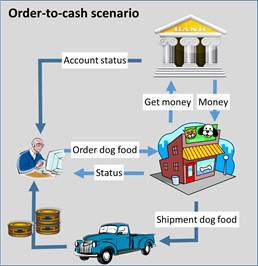
\includegraphics[width=0.6\linewidth] {Figures/Chapter5/Project/DogFoodShop.jpg}
	\caption[Order-to-cash scenario in a federation of enterprises and applications (simplified)]{Order-to-cash scenario in a federation of enterprises and applications (simplified)}
	\label{fig:DogFoodShop}
\end{figure}

Developing such a mutually adjusted solution by a federation of independent enterprises requires a project management approach different from traditional software development projects taking a process perspective (cf. \cite{book:ProjectHistory}). Therefore our focus is on how to implement loosely coupled systems for exchanging information between independent partners, rather than tightly coupled solutions for sharing information or other resources.
The section is structured as follows. First software development methodology and its elements are reviewed with respect to developing federated systems. This leads to our proposal of a software development approach for federated systems based on subject orientation.
\\
\subsection{Background}

\subsubsection{\textbf{Recommendations for creating federated systems}}
When independent enterprises develop a federated system a lot of managerial and technological aspects have to be considered, particularly with respect to managing collaborative business processes. This is reflected in the following recommendations (cf. \cite{book:PMThirdWave} , \cite{ChallengesDistPM} ):
\begin{enumerate}
	\item Start the foundation of a federation and identify members.
	\item Identify and describe the business services that organizations can provide or they need from partners in service level agreements.
	\item Harmonize the enactment of collaboration by coordinating the participating organizations according to defined business processes and identify the systems required for the federation.
	\item Integrate the identified and implemented services/systems into the intended application.
	\item Maximize the autonomy of organizations when collaborating, thereby ensuring organizations to benefit most from their own business objectives.
	\item Represent the partnerships between collaborating organizations when collaborating, and update changes in partnership.
	\item Guarantee the business privacy of organizations in the course of collaboration.
	\item Allow partners and other third parties to monitor, measure, and oversee the execution of business processes.
\end{enumerate}


\subsubsection{\textbf{Federation of enterprise information systems}}
\cite{article:VirtualEnterprise} define virtual enterprises and federations of enterprise information systems as follows: "\textit{The Enterprise partners' Virtual Enterprise (EP VE) is the federation of partners in the community that come together to achieve the goal of a federated distributed system environment, sharing their resources, and collaborating to achieve a common goal: the Federated System VE (FS VE). The partners in the federation retain autonomy over their resources, deciding which resources (personnel, resource dollars, equipment, etc.) are sharable for achieving this goal. The results of this VE are then useable by the partners in furthering their individual systems. The FS VE is seen to be a virtual system of distributed processing components (hardware and software), which are physically implemented and managed by the partners. It is a federation of the partners' systems, where each system retains its autonomy over all processing system components and sharable data/information. Retaining autonomy means defining which data or information and software/hardware assets will participate in the federation and be accessible and usable by other systems in the federation.}"\\
The definition shows that the focus is on sharable resources. This means when setting up a federation the VE members need to clarify ownership of the shared resources as well as access rights and the rights to change those. Such an approach often implies tight coupling of the involved enterprises and the related resources. Entities leaving a federation then cause difficulties with respect to separating involved systems (changing access rights) and sorting out ownership of information.
Alternatively, information can be exchanged between the partners by messages, implying only a loose coupling of the involved systems. In this case the partners only need to agree upon structure and meaning of the data, e.g., using XML schemes, and upon the implementation of the message exchange, e.g., by web services.
\\
\subsubsection{\textbf{Software development methodology}}
\textit{"A software development methodology is a collection of procedures, techniques, tools and documentation aids which help developers to implement software systems"}  \cite{book:ISDevelopment}. It may include modeling concepts, tools for model-driven architecture, integrated development environments (IDEs) etc. The so-called magic triangle (see figure \ref{fig:Triangle}) summarizes the various aspects of a software development methodology \cite{book:SoftEng}.

\begin{figure}[htbp]
	\centering
	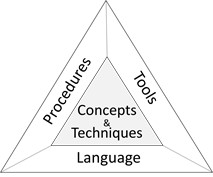
\includegraphics[width=0.6\linewidth] {Figures/Chapter5/Project/Triangle.jpg}
	\caption[Magic triangle of software development methodologies]{Magic triangle of software development methodologies}
	\label{fig:Triangle}
\end{figure}

Concepts and Techniques are used to create models of the software to be implemented, and are thus significantly influencing which languages, procedures and tools are utilized. The applied concept implies the artifacts to be produced, of which the executable software system is the most important one. The Language is used to create the artifacts and tools. Procedures describe the sequence in which the activities for creating the various artifacts are executed. While languages and tools can be replaced without impacting concepts and procedures, the latter are decisively determining the shape of a software development environment.
\\
\subsubsection{\textbf{Modeling concepts}}
Developing a federated system like the dog food store requires modeling cross-company business processes and the entities performing activities in these processes.
\paragraph{Business process modeling}
There are various approaches for specifying business process models. IT implementations of those models are called process-controlled applications [7] or workflows. The modeling approaches can be distinguished in three classes: (i) Control flow-based specifications put the focus on the activities. (ii) Object-based models mainly describe business objects and the sequence of operations to manipulate them. (iii) Communication-based models focus on the active entities in a process which exchange messages in order to coordinate their work.
By their nature the latter are promising candidates for modeling federations of systems. Business Process Model and Notation (BPMN), the currently most widely discussed modeling language, contains elements for the description of control flows and communication in business processes. In the following we discuss its communication-oriented features.
To model communication BPMN provides so-called pools, each representing a process that can exchange messages with processes in other pools. Conversation diagrams are the means to describe this mechanism: However, they do not allow specifying the sequence in which messages are exchanged. Although the sequence can be captured by collaboration diagrams, the semantics of sending and receiving messages is not precisely defined. For instance, it remains unclear whether messages are exchanged synchronously or asynchronously. Additionally a certain message from a pool can only be received in a single activity state, but not in other states. Choreography diagrams in BPMN also define the allowed message sequence between pools. [8] describe a choreography-based tool for specifying global processes. The problem is that choreography specifications cannot contain data. As a consequence a modeler can only describe message sequences being covered by regular expressions, which is the lowest level in the Chomsky hierarchy. This fact makes it impossible to model a behavior like the following: Pool S sends n messages of a type X to pool R. After that S sends a message Y to R. Subsequently S expects m messages of type A from pool R, which received the n messages of type X. The reason for that is that the messages cannot be counted, because data are not allowed in BPMN choreographies.
Given these properties of BPMN this notation has significant draw backs for modeling communication, hindering the precise development of federations of systems.

\paragraph{Multi-agent systems modeling}
The term agent has multiple meanings. We follow the definition given in [9]: An agent is an entity that performs a specific activity in an environment of which it is aware and that can respond to changes. A multi-agent system (MAS) is a system where several, perhaps all, of the connected entities are agents. The most important property of agents is their controlled autonomy: They independently execute their role-specific behavior, and in multi-agent systems they communicate with each other. These properties are alike those of federated systems which therefore can be considered as multi-agent systems. This means that software development methodologies for agent-oriented software (for an overview see [8]) can help developing federations of applications.
\\
\subsubsection{\textbf{Procedures}}
Software Life Cycles (SLC) build a framework for software development procedures. All software development projects follow a series of phases. While software life cycles can be defined in many different ways, each of them comprises the following generic activities:
\begin{list}{-}{spacing}
	\item Project conception or initiation
	\item Planning
	\item Execution with specification and implementation activities
	\item Termination
\end{list}

In the traditional waterfall approach these activities are performed in the sequence shown above. Other life cycle concepts propose overlapping the development steps, suggest alternatives like the V model or agile development procedures like Extreme Programming and Scrum. \cite{article:ObjectOrientedSWdev}, \cite{book:SoftEng} and \cite{book:ISDevelopment} give an overview of the various approaches.
\\
\subsubsection{\textbf{Work break down structure (WBS)}}
The work break-down structure describes the artifacts to be created in a project in a hierarchical way. A work break-down structure element may be a product, data, service, or any activity results contained in the software life cycle or any combination thereof. A WBS also provides the necessary framework for detailed cost estimating and control along with guidance for schedule development and control. The top level of the WBS should identify the major phases and milestones of the project in a summative fashion. Consequently, the phases used in the top level depend on the software development methodology applied in a project. The first level can either represent the phases used in the software life cycle or the major artifacts of the system to be developed. In case the top level is SLC-oriented it might be built by requirement specification, software architecture, programming, test etc. In the case of an evolutionary life cycle there will be topics like Release 1, Release 2 etc., followed by headlines like requirement specification on the second level.
Another alternative is to use top level headlines corresponding to artifacts created by modeling activities, such as 'create communication structure' or 'describe subject behavior'.
\\
The WBS is created during the planning phase of a project life cycle. During this phase the project manager works with the project team to make sure that the client's needs are addressed and the project is planned completely and approved by the client prior to any sort of production beginning on the project.

\subsubsection{Organisational break down structure and software architecture}
An organizational breakdown structure (OBS) complements the WBS and resource breakdown structure of a project. Project organizations can be broken down in much the same way as the work or product. The OBS is created to reflect the strategy for managing the various aspects of the project and shows the hierarchical breakdown of the management structure. Hence, the work break down structure has a significant impact on the organizational structure of the project team. The same holds for the phases of the software life cycle and the system architecture influencing the work break down structure. Conway’s law states “organizations which design systems ... are constrained to produce designs which are copies of the communication structures of these organizations” \cite{article:ConwaysLaw}. A variation of Conway’s law can be found in [12]. "If the parts of an organization (e.g., teams, departments, or subdivisions) do not closely reflect the essential parts of the product, or if the relationship between organizations do not reflect the relationships between product parts, then the project will be in trouble... Therefore: Make sure the organization is compatible with the product architecture” \cite{book:OrgPatternsAgile}.
As we look at developing federations of systems with a federation of independent project teams, the system architecture needs to be aligned with the multiple project team structure.
\\

\subsection{Software Development Methodology For Federated Systems}
The software development methodology for federated systems proposed here is based on Subject-oriented Business Process Management (S-BPM)


\subsubsection{Development as a multiple-team structure}
We now assume that the dog food order-to-cash scenario does not yet exist. The store wants to extend its services for the customers by offering online shopping and home delivery. In order to reach this business objective it takes the initiative to found a federation of enterprises which combine their services and develop a corresponding federation of systems.
Each federated enterprise establishes a project team, working on their parts of the solution independent from each other. This leads to a multiple-team project on the federation level \cite{book:OrgPatternsAgile}. As the teams belong to different, independent companies they all have their own development culture and methodology.
Since there is no single line management who can assign an overall project manager, the federation members need to agree on a project leader and the competencies related to this role. As the initiator of a federation has the most interest in the development of the federated solution it might be helpful that this company, in our case the store, recruits the leader.

His or her major task is to ensure smooth communication between the independent teams, respectively their managers. The project teams needs to coordinate how the systems they are developing communicate with each other. Their major communication paths are predefined by the communication structure of the system federation. This strategy leads to a high socio-technical-congruence. Figure \ref{fig:Multiple-team} (CS: no missing) shows the team and communication structure of the dog food order-to-cash federation.

\begin{figure}[htbp]
	\centering
	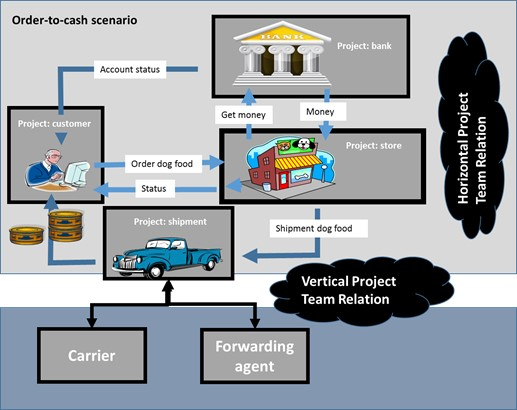
\includegraphics[width=0.6\linewidth] {Figures/Chapter5/Project/MultipleTeam.jpg}
	\caption[Multiple-team project and its communication structure]{Multiple-team project and its communication structure}
	\label{fig:Multiple-team}
\end{figure}

Beside that top-level communication implied by the problem structure, each team can use services offered by other enterprises. Figure 6 reveals that the shipment company uses the service of carriers and forwarding agents, in order to implement the transportation service offered to the dog food shop. This communication relation is of no interest for other federation members and thus should not be visible to the top level teams. It belongs to the internal issues of the shipment project team.
\\
\subsubsection{Development process for federated systems}
 The artifacts to be created according to subject orientation need to be developed by a federation of teams related to the subject interaction structure.

\paragraph{Specification of the communication structure}\
The communication between the various members of the federation needs to be specified in more detail. This is done by assigning a subject to each member of the federation and defining the messages exchanged between the subjects. Together with the data transported by the messages a communication model of the system federation is defined. The advantage of the subject-oriented approach is that the system communication structure is directly in line with the communication structure of the corresponding developing teams. The result of that step is the subject interaction diagram (SID).

\paragraph{Specification of the subject behaviour}\
After defining the communication structure the behavior of each subject is specified. The modelers describe the allowed sequence of messages exchanged on top level and the internal functions of the individual systems. These internal functions represent the services executed by the corresponding federation partner either directly or supported by other service providers. They also encapsulate the communication with those sub-contractors as it is of no interest on the top level of the federation.\\
The behavior of a subject is mainly defined by the corresponding project team, however, in close coordination with the teams responsible for the partner subjects. The teams only need to make sure a message sent to a partner has a receive state in the corresponding subject behavior and vice versa. This pairwise coupling means, e.g., that the behavior description of the shipment company has to contain a state for receiving the “Transfer order” message, transmitted by the related send state in the behavior diagram of the dog food store subject. In order to correctly model these interactions the responsible project teams need also to agree on the interaction sequence of the subjects. However, their internal task behavior (i.e. sequence of functions for task accomplishment) might not become visible to others, as is specified decentralized and might not be shared at all.

\paragraph{Implementation of the input pool}\
The input pool is the abstract concept for defining the semantics of message exchange. Partners exchanging messages need to agree on how they implement the input pool semantics. Sending requires the sending subject to execute a function to deposit a message in the input pool of the receiver. For each subject doing so an implementation agreement is necessary. Since an input pool is owned by exactly one subject, the functionality for accessing it is local and does not need to be coordinated with the partners. In most cases input pools are implemented as web services.

\paragraph{Implementation of subject behaviour}\
Each team has to implement the behavior of its subject. This means they have to ensure that depositing and removing messages (including business objects) in or from the input pool are executed and internal functions are invoked in the specified sequence. Workflow engines are appropriate tools for implementing that functionality.\

\paragraph{Implementation of internal functions}\
The internal functions realize the kernel of the service contributed by a partner to a federated application. Messages are the means to cause the invocation of an internal function, and they transport its result to a partner subject. Internal functions can be based on existing systems, e.g., an SAP client.  They also can be implemented using another federated solution, or being developed from scratch. The way an internal function is realized is a local decision taken by the corresponding project team.

\paragraph{Operation of a federated system}\
Beside the development and deployment the non-functional aspects of a federated system need to be agreed upon by the contributing partners. For this purpose they negotiate service level agreements (SLA) defining response time, down time, reaction time in error cases etc. The SLA also includes business aspects like costs and regulations for exceptional situations like a member leaving the federation and bringing in another one.

\subsubsection{\textbf{Federated work break down structure}}
The various activities described so far can be organized in a federated work break-down structure as shown in figure \ref{fig:WBSDog}.

\begin{figure}[htbp]
	\centering
	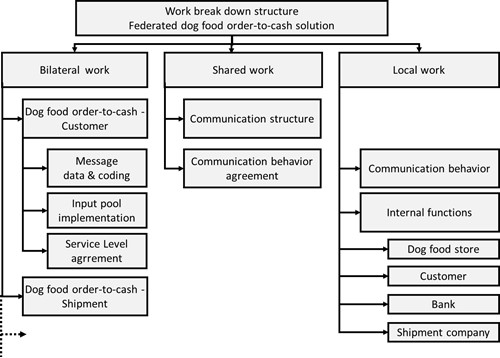
\includegraphics[width=0.6\linewidth] {Figures/Chapter5/Project/WBSDog.jpg}
	\caption[Work break down structure for the development of a federated system]{Work break down structure for the development of a federated system}
	\label{fig:WBSDog}
\end{figure}

The tasks can be divided into three types:
\textbf{Joint work} concerns the top level of the federation and therefore is done collaboratively by all members of a federation. The major issue on this level is to agree on communication structure and behavior of the entire system, while the behavior of each subject can be described individually by the corresponding member of the federation.\\
\textbf{Some work can be done bilateral}. Communicating partners, e.g., agree on the coding of the business objects and the implementation of the input pool. They also define the service level agreements.\\
\textbf{Local work} comprises activities of the development teams which do need to be coordinated with teams of other federation members. A major example in this context is the set of internal functions of each subject, being a local matter, and developed following the particular culture and methodology of the respective team.
\\


\subsection{Conclusion}
We have presented an approach for developing federated systems. The concept considers the characteristics of virtual enterprises combining the services of the partners to satisfy customer needs while keeping legal, organizational, technological and cultural independence.
Our communication-oriented view follows the idea that the decentralized structure of federated systems needs to be reflected in the organizational structure of multiple project teams for developing such systems. Those teams belong to separate enterprises and are mutually independent with respect to methodology, technology etc. they use to develop their individual part of the federated system.
The proposed approach establishes a layer above the enterprise-specific environments. It helps building coherence on the top level of the federated system solution, while the teams, system elements etc. on the individual level of each federation member keep the highest degree of independence.

\subsection{Future Work}
It has to be investigated whether the OWL definition and/or the execution semantics has to be adapted for a better project management support. Based on that results some guidelines for a subject oriented project management has to be developed and enhanced based on practical experiences.